{\let\clearpage\relax \chapter{图和表}}

\section{插图}

\section{array宏包}

数组宏包\qd{array}改进和扩展了\LaTeX 的\qd{tabular、tabular*、array}环境的功能,增强了\qd{列格式}的功能和一些其他表格参数的调整功能。

\begin{table}[!ht]
	\caption{array宏包基本参数}
	\begin{center}
	\begin{tabular}{|c|c|}
	\hline 
	选项	&	说明 \\ 
	\hline
	l	&	左对齐 \\ 
	\hline
	c	&	居中 \\ 
	\hline
	r	&	右对齐 \\ 
	\hline
	p\{列宽\}	&	顶对齐 \\ 
	\hline
	m\{列宽\}	&	居中对齐 \\ 
	\hline
	b\{列宽\}	&	底对齐 \\ 
	\hline
	@\{声明\}	&	该列每行都插入声明中的文本 \\ 
	\hline
	>\{声明\}	&	命令或需要插入列元素前的文本 \\ 
	\hline
	<\{声明\}	&	命令或需要插入列元素后的文本 \\ 
	\hline
	|	&	在列边或列间插入垂直线 \\ 
	\hline
	!\{声明\}	&	在列间插入声明要求的样式 \\ 
	\hline
	\end{tabular}
\end{center}
\end{table}

\section{浮动体}

浮动体将图或表与其标题定义为整体,然后动态排版,以解决图、表卡在换页处造成的过长的垂直空白的问题。但有时它也会打乱你的排版意图,因此使用与否需要根据情况决定。图片的浮动体是\qd{figure}环境,而表格的浮动体是\qd{table}环境。

对表格来说,输出表格内容的是\qd{tabular}环境,\qd{table}只是一个会浮动体(到处乱跑的盒子)而已。没有\qd{tabular}环境,\qd{table}环境一样会乱跑;没有\qd{table}环境,\qd{tabular}环境一样会输出表格内容。

下面是一个典型的浮动体例子。参数\qd{!htb}含义是:! 表示忽略内部参数(比如内部参数对一页中浮动体数量的限制);h、t、b 分别表示插入此处、插入页面顶部、插入页面底部,故htb表示优先插入此处,再尝试插入到某页顶,最后尝试插入到页底。此外还有参数p,表示允许为浮动体单独开一页。\LaTeX 的默认参数是tbp。请不要单独使用htbp中的某个参数,以免造成不稳定。另外需要注意的是\qd{label}命令写在\qd{caption}命令下方,否则交叉引用会出现问题。

\begin{latex}{}
\begin{table }[!htb]				%浮动体环境
	\begin{center}					%居中环境
		\caption{标题}
		\label{用于交叉引用的标签}
		\begin{tabular }{}			%表格环境
		\end{tabular}
	\end{center}
\end{table}
\end{latex}

\section{表格}
\LaTeX 原生的表格功能非常有限,甚至不支持单元格跨行和表格跨页,我们必须通过宏包来解决。如有需求,可在\qd{tabular}环境外定义全部表格线的粗细,例如,\verb|\setlength{\arrayrulewidth}{2pt}|或者直接写\verb|\arrayrulewidth=2pt|。

\begin{codeshow}
\centering
\arrayrulewidth=1pt%表格线宽度
\begin{tabular}
	{|C{6mm}|C{6mm}|C{6mm}|}
	\hline
	\multicolumn{3}{|c|}{整体表格线宽}\\
	\hline
	7&5&3\\
	\hline
	6&1&8\\
	\hline
\end{tabular}
\end{codeshow}

如果需要单独定义某一条表格线的粗细,必须要做额外的设置。

如果我们要更改\qd{垂直表格线}的粗细,可以利用\qd{array}宏包提供的新列格式选项定义命令。其中的新选项名只能用一个字母来表示。使用该命令更改中间两条垂直线粗细为2pt。

\begin{latex}{}
\newcolumntype{新选项名称}[参数数量]{列格式}
\newcolumntype{I}{!{\vrule width 4pt}}
\end{latex}

\begin{codeshow}
	\centering
	\newcolumntype{I}
		{!{\vrule width 2pt}}
	\begin{tabular}
		{|C{6mm}IC{6mm}IC{6mm}|}
		\hline 
		\multicolumn{3}{IcI}{垂直线粗细}\\
		\hline 
		7&5&3\\
		\hline 
		6&1&8\\
		\hline
	\end{tabular}
\end{codeshow}

水平表格线的粗细较难修改,需要使用\qd{booktabs}宏包,该宏包可以任意修改水平线粗细,还可以在其上、下方附加一段垂直空白。

\begin{codeshow}
	\centering
	\begin{tabular}
		{|C{8mm}|C{8mm}|C{8mm}|}
		\hline 
		\multicolumn{3}{|c|}{水平线宽}\\
		\specialrule{2pt}{0pt}{0pt}
		7&5&3\\
		\hline
		6&1&8\\
		\hline
	\end{tabular}
\end{codeshow}

\qd{array}包重新实现了\qd{tabular}环境,加了不少新选项进去。比如我们可以定义\qd{F}为一个居中且在数学环境中的列类型。然后在\qd{tabular}中调用\qd{F}即可在表格环境中排出数学样式。

\begin{codeshow}
\centering
\newcolumntype{F}{>{$}c<{$}}
\begin{tabular}{FFF}
	\alpha & \beta    & \gamma   \\
	\delta & \epsilon & \upsilon \\
	\sigma & \tau     & \phi     \\
\end{tabular}
\end{codeshow}

\subsection{跨行和跨列表格}

既跨行又跨列时,必须把\qd{multirow}命令放在\qd{multicolumn}内部,始终记住跨列享受最高的优先级。

\begin{codeshow}
\centering
\begin{center}
	\begin{tabular}{|c|c|c|}
		\hline
		\multirow{2}{2cm}{A Text!}
		& ABC & DEF \\
		\cline{2-3} & abc & def \\
		\hline
		\multicolumn{2}{|c|}
		{\multirow{2}*{Nothing}} & XYZ \\
		\multicolumn{2}{|c|}{} & xyz \\
		\hline
	\end{tabular}
\end{center}
\end{codeshow}

\begin{codeshow}
	\centering
	\begin{tabular}{|ccc|}
		\hline
		2&9&4\\
		7&\multicolumn{2}{c|}
			{\multirow{2}*{{?}}}\\
		6&&\\
		\hline
	\end{tabular}
\end{codeshow}

\subsection{彩色表格}

彩色表格。该宏包主要使用的命令是\qd{columncolor}和\qd{rowcolor},一个用来给列进行着色,一个是给行进行着色,下面这个例子已经全部涉及到了。

\begin{codeshow}
	\centering
	\begin{tabular}{ccc}
		\rowcolor[gray]{.9}
		2&9&4\\
		\rowcolor[gray]{.8}
		7&5&3\\
		\rowcolor[gray]{.7}
		6&1&8\\
	\end{tabular}
\end{codeshow}

\begin{codeshow}
	\centering
	\begin{tabular}%
		{>{\columncolor[gray]{.9}}c%
		>{\columncolor[gray]{.8}}c%
		>{\columncolor[gray]{.7}}c}
		2&9&4\\
		7&5&3\\
		6&1&8\\
	\end{tabular}
\end{codeshow}

\begin{codeshow}
	\centering
	\begin{tabular}{ccc}
		\cellcolor[rgb]{.9,.9,.9}2&
		\cellcolor[rgb]{.8,.9,.9}9&
		\cellcolor[rgb]{.7,.9,.9}4\\
		\cellcolor[rgb]{.9,.8,.9}7&
		\cellcolor[rgb]{.8,.8,.9}5&
		\cellcolor[rgb]{.7,.8,.9}3\\
		\cellcolor[rgb]{.9,.7,.9}6&
		\cellcolor[rgb]{.8,.7,.9}1&
		\cellcolor[rgb]{.7,.7,.9}8\\
	\end{tabular}
\end{codeshow}

一个复杂的彩色表格例子,代码留着以后仔细看,彩色表格应该用的不多。

\begin{latex}{}
%使用array宏包的特性来定义几个表格属性,只适用于本环境
\newcommand*{\arraycolor}[1]{\protect\leavevmode\color{#1}}
\newcolumntype{A}{>{\columncolor{blue!50!white}}c}
\newcolumntype{B}{>{\columncolor{LightGoldenrod}}c}
\newcolumntype{C}{>{\columncolor{FireBrick!50}}c}
\newcolumntype{D}{>{\columncolor{Gray!42}}c}
\begin{center}
	\sffamily
	\arrayrulecolor{white}
	\arrayrulewidth=1pt
	\renewcommand{\arraystretch}{1.5}
	\rowcolors[\hline]{3}{.!50!White}{}
	\begin{tabular}{A|B|C}
		\multicolumn{3}{D}{\bfseries Example table}\\
		\rowcolor{.!50!Black}
		\arraycolor{White}\bfseries First column &
		\arraycolor{White}\bfseries Second column&
		\arraycolor{White}\bfseries Third column\\
			1 & A & E\\
			2 & B & F\\
			3 & C & G\\
			4 & D & H\\
	\end{tabular}
\end{center}
\end{latex}

%\begin{table}[!ht]
%	\centering
%	%使用array宏包的特性来定义几个表格属性,只适用于本环境
%	\newcommand*{\arraycolor}[1]{\protect\leavevmode\color{#1}}
%	\newcolumntype{A}{>{\columncolor{blue!50!white}}c}
%	\newcolumntype{B}{>{\columncolor{LightGoldenrod}}c}
%	\newcolumntype{C}{>{\columncolor{FireBrick!50}}c}
%	\newcolumntype{D}{>{\columncolor{Gray!42}}c}
%		\sffamily
%		\arrayrulecolor{white}
%		\arrayrulewidth=1pt
%		\renewcommand{\arraystretch}{1.5}
%		\rowcolors[\hline]{3}{.!50!White}{}
%		\begin{tabular}{A|B|C}
%			\multicolumn{3}{D}{\bfseries Example table}\\
%			\rowcolor{.!50!Black}
%			\arraycolor{White}\bfseries First column &
%			\arraycolor{White}\bfseries Second column&
%			\arraycolor{White}\bfseries Third column\\
%			1 & A & E\\
%			2 & B & F\\
%			3 & C & G\\
%			4 & D & H\\
%		\end{tabular}
%\end{table}


\subsection{斜线表头}

虽然斜线表头是不符合国标的,但在非正式场合用得还挺多的。制作斜线表头需要\qd{diagbox}宏包,刘海洋写的,中文说明。

\begin{codeshow}
	\centering
	\begin{tabular}{|l|ccc|}
		\hline
		\diagbox{Time}{Room}{Day}
			&Mon&Tue&Wed\\
		\hline
		Morning&used&used&\\
		Afternoon& &used&used\\
		\hline
	\end{tabular}
\end{codeshow}

\subsection{表格标题}

表格标题命令默认只能在浮动体内使用,在导言中添加如下命令,便可以在浮动体外使用\verb|\figcaption|和\verb|\tabcaption|命令来为图标添加标题。为了防止标题和图表不在一页,我们也可以用\verb|minipage|环境把它们包起来。

\begin{latex}{}
\makeatletter
\newcommand\figcaption{\def\@captype{figure}\caption}
\newcommand\tabcaption{\def\@captype{table}\caption}
\makeatother
\end{latex}

\begin{latex}{}
\begin{tabular}{|C{1cm}|C{1cm}|C{1cm}|}
	\hline
	\multirow{2}*{时间} & \multicolumn{2}{c|}{星期}\\
	\cline{2-3} & 一 & 二 \\
	\hline
	8:30 & 化学 & 物理\\
	9:30 & 韩语 & 数学\\
	\hline
\end{tabular}
\end{latex}

\begin{table}[!ht]
\centering
\caption{一张课表}
\begin{tabular}{|C{1cm}|C{1cm}|C{1cm}|}
	\hline
	\multirow{2}*{时间} & \multicolumn{2}{c|}{星期}\\
	\cline{2-3} & 一 & 二 \\
	\hline
	8:30 & 化学 & 物理\\
	9:30 & 韩语 & 数学\\
	\hline
\end{tabular}
\end{table}

\begin{figure}[!ht]
	\begin{center}
		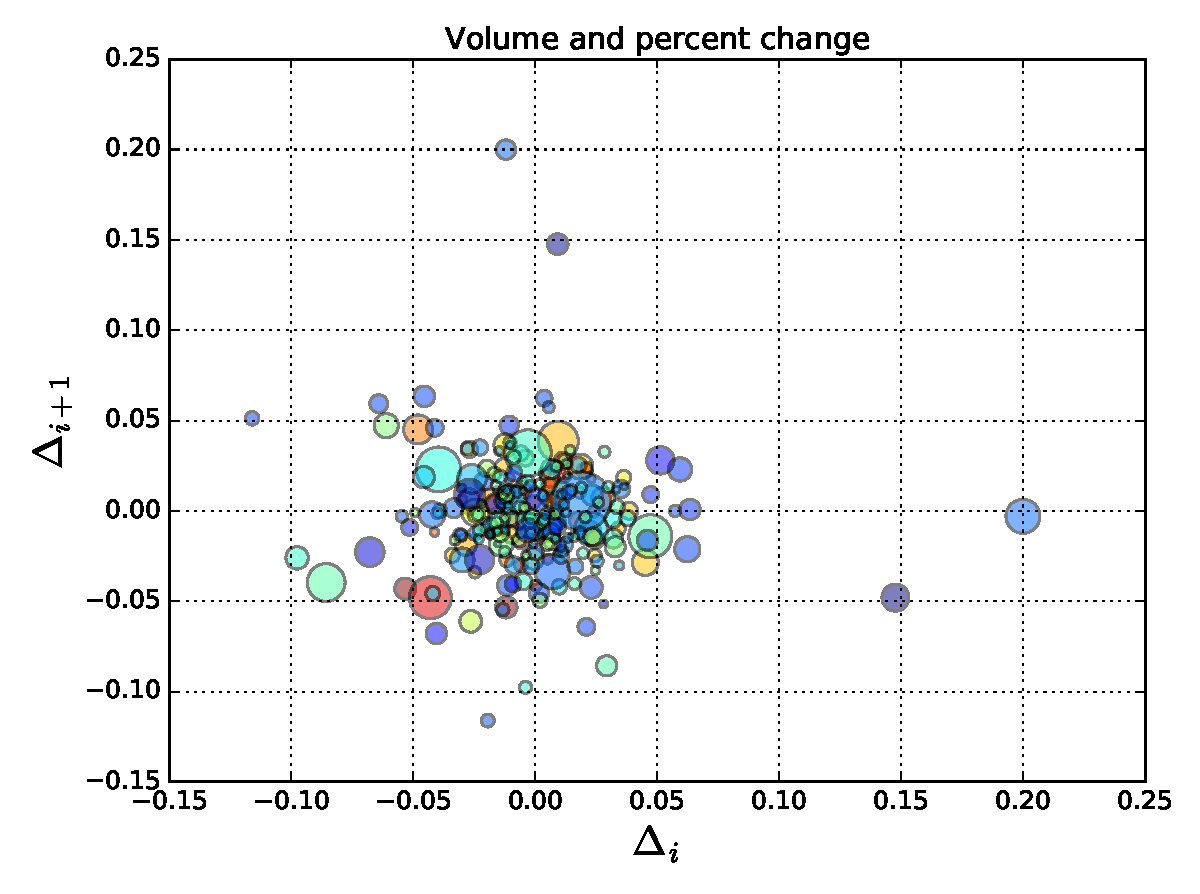
\includegraphics[width=10cm]{tabular-caption}
		\caption{一副图像}
	\end{center}
\end{figure}
